\chapter{Results}
\label{cha:validation}
\section{Test data set}
Evaluation of implemented prototype was performed using a set of textual process description with corresponding hand-made process diagram. This data set was introduced in article~\cite{friedrich-2011}. Thirty-two models from the introduced data set were used to evaluate proposed method. This subset contains the descriptions and models introduced in academic textbooks~(\cite{white-bpmn-reference-guide},~\cite{praxishandbuch}), BPMN modelling tutorials and industrial sources (websites and on-line help documentation of BPM tool vendors -- Active VOS, Oracle, and BizAgi). The academic models introduced in~\cite{friedrich-2011} were provided by a courtesy of the Humboldt Universit at zu Berlin, the Technishe Universit at Berlin, the Queensland University of Technology.

\section{Validation methodology}
The generated models were compared with hand-made models  in two ways:
\begin{itemize}
	\item using a set of complexity metrics introduced in several papers -- this way it is possible to numerically compare the structure of models,
	\item by manual analysis of hand-made and generated models.
\end{itemize}
The complexity metrics used in evaluation method were introduced in several articles. Those metrics are:
\begin{itemize}
	\item Number Of Activities in a process (\texttt{NOA}) and Number Of Activities and Control-flow elements (\texttt{NOAC}) were introduced by Cardoso et al. in~\cite{cardoso-metrics}. Those basic metrics simply returns information about number of basic process elements in process model -- activities, in case of \texttt{NOA} metric, activities and control flow elements (gateways , events) in case of \texttt{NOAC} metric. For the purpose of the proposed method evaluation, \texttt{NOAC} metric is not directly used -- rather, a variation of \texttt{NOAC}, which returns only a number of control flow elements is used. This metric will labelled \texttt{NOC} -- Number Of Control-flow elements. Using \texttt{NOA} and \texttt{NOC} metrics it is possible to compare number of activities and control flow elements separately,
	\item Coefficient of Network Complexity (\texttt{CNC}) metric introduced by Latva-Koivisto in~\cite{latva-metric}. \texttt{CNC} can be used to measure the degree of complexity of a critical pass network. The formula of CNC can be described by equation $ (number\_of\_arcs)/(number\_of\_activities\_joins\_and\_splits) $,
	\item Average Gateway Degree~(\texttt{Avg}) -- Average of the number of both incoming and outgoing arcs of the gateway
	nodes in the process model. This metric was introduced in~\cite{sanchez-metric},
	\item Gateway Heterogeneity~(\texttt{Heter}) -- Number of different types of gateways used in a model. This metric was introduced in~\cite{sanchez-metric}.
\end{itemize}
Using this set of the complexity metric, it should be possible to compare the structural differences between manually created and generated models. Additionally, the generated models were manually analysed and compared with hand-made models in order to find limitations and weaknesses of implemented method.

\section{Validation results}

\subsection{Metrics value analysis}
Detailed metrics values for each model are presented in tables~\ref{csv:metrics_part_one} and~\ref{csv:metrics_part_two}. Table~\ref{csv:metrics_part_one} presents the values of \texttt{NOA} and \texttt{NOC} metrics. This table is structured in this way:
\begin{itemize}
	\item first column shows a model name,
	\item columns number two to number four present values of \texttt{NOA} metric for hand-made model (column \texttt{NOA-H}), generated model (column \texttt{NOA-G}), difference between \texttt{NOA} metric for hand-made model and for generated model (column \texttt{NOA-diff}). Fifth column shows the proportion of difference between \texttt{NOA} metrics proportional to \texttt{NOA} metric for hand-made model (column \texttt{NOA-prop}),
	\item columns number six to number nine are organized in similar manner to previous part, but present values of \texttt{NOC} metric. Columns are named in the similar way (\texttt{NOC-H}, \texttt{NOC-G}, \texttt{NOC-diff}, \texttt{NOC-prop}).
\end{itemize}
Difference between metrics indicates whether the number of corresponding elements (activities or control flow elements) in the generated model were lower (when difference is positive number) or higher (when difference is a negative number) than in the hand-made model. Table~\ref{csv:noa_noc_max_min} shows the minimum and maximum values of metrics (with the name of corresponding model), listing difference and  proportional difference separately.
\newpage
{\scriptsize
	\begin{longtable}{|p{0.09 \hsize}|p{0.08 \hsize}|p{0.08 \hsize}|p{0.08 \hsize}|p{0.08 \hsize}|p{0.08 \hsize}|p{0.08 \hsize}|p{0.08 \hsize}|p{0.09 \hsize}|}
		\hline
		Model name & NOA-H & NOA-G & NOA-diff & NOA-prop & NOC-H & NOC-G & NOC-diff & NOC-prop
		\\\hline\hline
		\csvreader[late after line=\\\hline]
		{./results/metrics_part_one.csv}
		{Model name=\CA,NOA-H=\CB,NOA-G=\CC,NOA-diff=\CD,NOA-prop=\CE,NOC-H=\CF,NOC-G=\CG,NOC-diff=\CH,NOC-prop=\CI}
		{\CA & \CB & \CC & \CD & \CE & \CF & \CG & \CH & \CI}
		\caption{Validation results -- NOA and NOC metrics}
		\label{csv:metrics_part_one}
	\end{longtable}
}
\begin{table}[H]
	{\small
	\centering
	\begin{tabular}{|p{0.14 \textwidth}|p{0.15 \textwidth}|p{0.2 \textwidth}|p{0.15 \textwidth}|p{0.2 \textwidth}|}
		\hline
		Metric & Min. difference & Model & Max. difference & Model \\
		\hline
		NOA & -47 & Model 5 & 1 & Model 31 \\
		\hline
		NOA (prop.) & -380.00\% & Model 18 & 12.50\% & Model 31 \\
		\hline
		NOC & -4 & Model 18 & 28 & Model 5 \\
		\hline
		NOC (prop.) & -200.00\% & Model 18 & 90.32\% & Model 6 \\
		\hline
	\end{tabular}
	}
	\caption{Minimum and maximum values of NOA and NOC metrics}
	\label{csv:noa_noc_max_min}
\end{table}
Analysis of results shown in tables~\ref{csv:metrics_part_one}~and~\ref{csv:noa_noc_max_min} shows that most of the generated models have higher number of activities (higher \texttt{NOA} metric) and lower number of control flow elements (lower \texttt{NOC} metric) than the hand-made models. Average of proportional difference between \texttt{NOA} metrics equals to $ -87.50\% $. Average of difference between \texttt{NOC} metrics equals to $ 31.74\% $. Model number eighteen is an extreme case, having nearly five times more activities than corresponding hand-made models -- while the hand-made model have only five activities, the generated model consists of twenty four activities. In case of \texttt{NOC} metric, the extreme values are a bit confusing. While the lowest proportional difference is $ -200\% $, meaning that the generated model has three times more of control flow elements than hand-made model, the actual numbers of control flow elements are two (in case of hand-made model) and six (in case of generated model). In most cases, the hand-made model consists of more control flow elements than the generated one.\\
To summarize the analysis of \texttt{NOA} and \texttt{NOC} metrics:
\begin{itemize}
	\item in case of \texttt{NOA} metric, the generated models had higher value of this metric in twenty nine cases, equal value to the hand-made model in two cases (models number three and twenty-eight) and lower value in one case (model number thirty-one),
	\item in case of \texttt{NOC} metric, the generated models had higher value of this metric in two cases (models number sixteen and eighteen), equal value to the hand-made model in six cases (models number seven, nine, thirteen, seventeen, twenty and twenty-four) and lower value in twenty-four cases.
\end{itemize}
\begin{figure}[p]
	\centering
	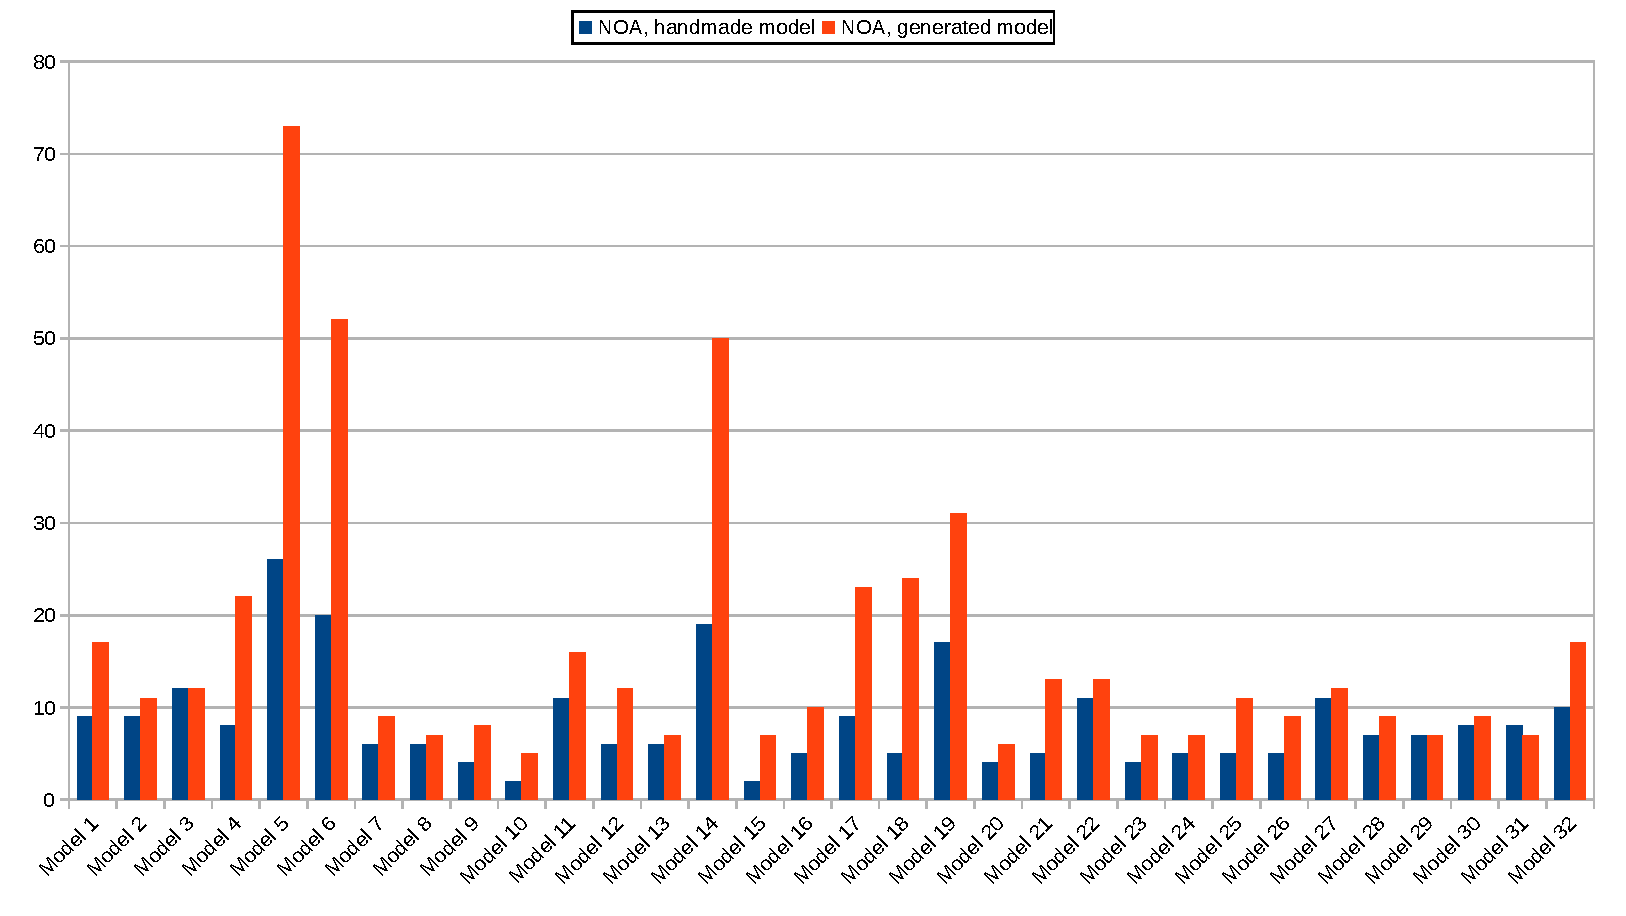
\includegraphics[width=0.95\textheight, angle=90]{./images/noa_chart.pdf}
	\caption{Chart showing comparison of NOA metric between models}
	\label{bpmn:noa_chart}
\end{figure}
\begin{figure}[p]
	\centering
	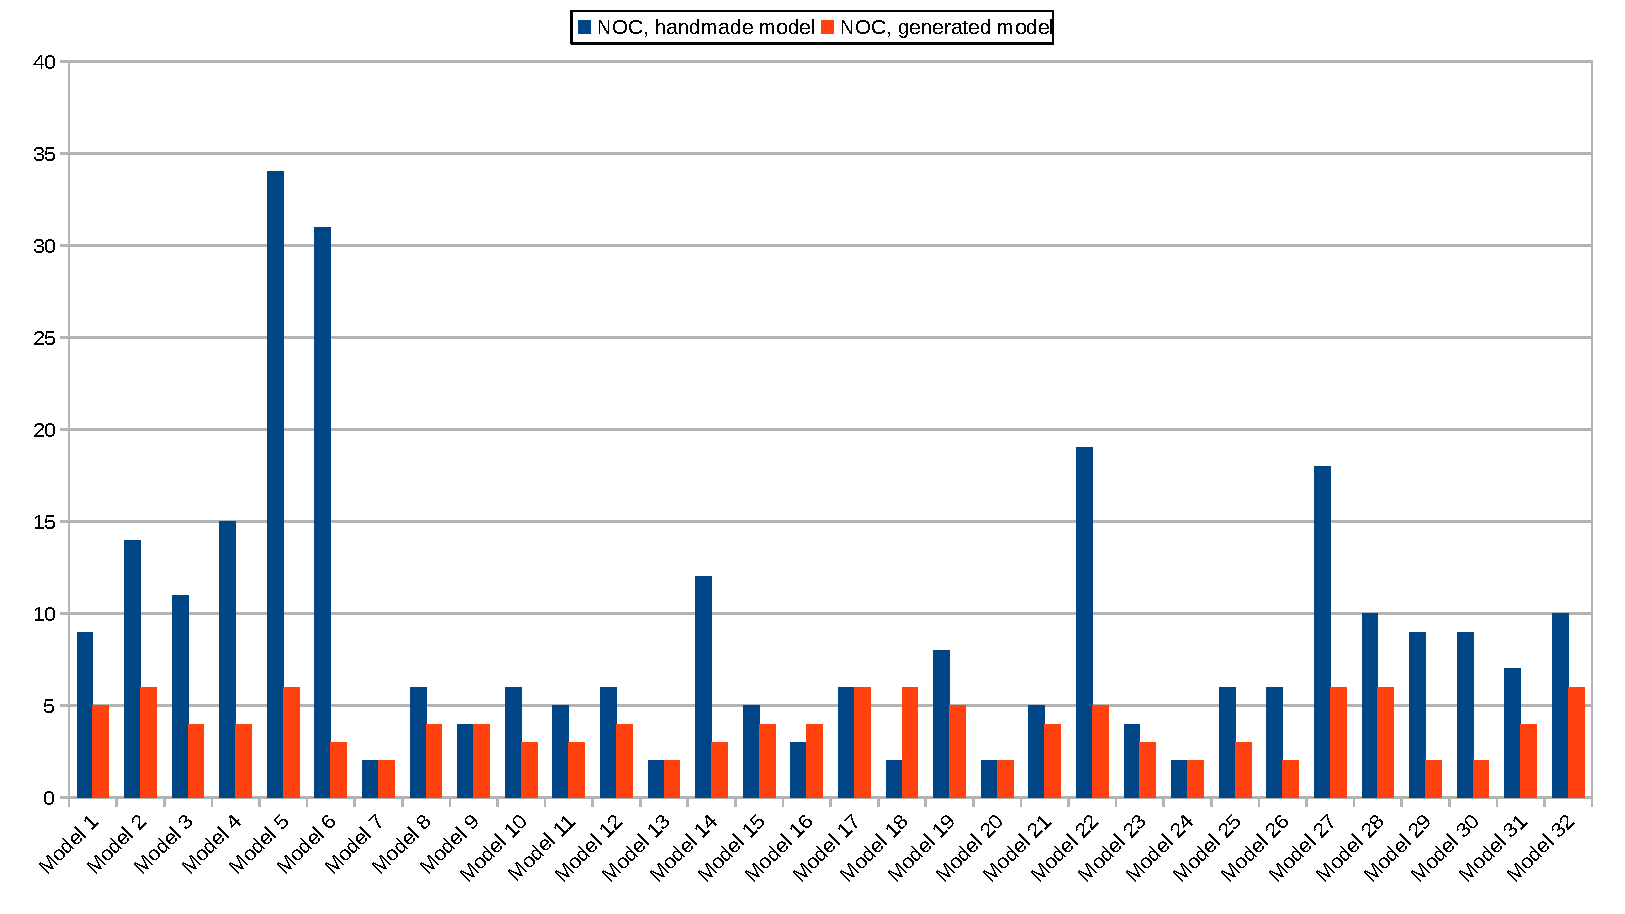
\includegraphics[width=0.95\textheight, angle=90]{./images/noc_chart.pdf}
	\caption{Chart showing comparison of NOC metric between models}
	\label{bpmn:noc_chart}
\end{figure}
Table~\ref{csv:metrics_part_two} presents the values of Coefficient of Network Complexity, Average Gateway Degree and Gateway Heterogeneity metrics. This table is structured in this way:
\begin{itemize}
	\item first column shows a model name,
	\item columns number two to number four present values of \texttt{CNC} metric for hand-made model (column \texttt{CNC-H}), generated model (column \texttt{CNC-G}), absolute difference between \texttt{CNC} metric for hand-made model and for generated model (column \texttt{CNC-diff}),
	\item columns number five to number seven are similar to previous part but present values of Average Gateway Degree metric. Columns are named in the similar way (\texttt{Avg-H}, \texttt{Avg-G}, \texttt{Avg-diff}),
	\item columns number five to number seven are similar to previous part but present values of Gateway Heterogeneity metric. Columns are named in the similar way (\texttt{Heter-H}, \texttt{Heter-G}, \texttt{Heter-diff}).
\end{itemize}
\newpage
{\scriptsize
	\begin{longtable}{|p{0.09 \hsize}|p{0.07 \hsize}|p{0.07 \hsize}|p{0.08 \hsize}|p{0.07 \hsize}|p{0.07 \hsize}|p{0.08 \hsize}|p{0.07 \hsize}|p{0.07 \hsize}|p{0.07 \hsize}|}
		\hline
		Model name & CNC-H & CNC-G & CNC-diff & Avg-H & Avg-G & Avg-diff & Heter-H & Heter-G & Heter-diff
		\\\hline\hline
		\csvreader[late after line=\\\hline]
		{./results/metrics_part_two.csv}
		{Model name=\CA,CNC-H=\CB,CNC-G=\CC,CNC-diff=\CD,Avg-H=\CE,Avg-G=\CF,Avg-diff=\CG,Heter-H=\CH,Heter-G=\CI,Heter-diff=\CJ}
		{\CA & \CB & \CC & \CD & \CE & \CF & \CG & \CH & \CI & \CJ}
		\caption{Validation results -- Coefficient of Network Complexity, Average Gateway Degree and Gateway Heterogeneity metrics}
		\label{csv:metrics_part_two}
	\end{longtable}
}
\begin{table}[H]
	{\small
	\centering
	\begin{tabular}{|p{0.2 \hsize}|p{0.15 \hsize}|p{0.15 \hsize}|p{0.1 \hsize}|p{0.15 \hsize}|p{0.1 \hsize}|}
		\hline
		Metric & Avg. difference & Min. difference & Model & Max. difference & Model \\
		\hline
		CNC & 0.019 & -0.305 & Model 27 & 0.591 & Model 26 \\
		\hline
		Avg. Gateway Degree & 0.058 & -4.000 & Model 18 & 3.000 & Model 26 \\
		\hline
	\end{tabular}
	}
	\caption{Average, minimum and maximum values of Coefficient of Network Complexity and Average Gateway Degree metrics}
	\label{csv:cnc_avg_heter_max_min}
\end{table}
Analysis of results shown in tables~\ref{csv:metrics_part_two}~and~\ref{csv:cnc_avg_heter_max_min} shows that differences in values of Coefficient of Network Complexity and Average Gateway Degree metrics do not differ significantly between hand-made and generated models. The average difference of \texttt{CNC} equals to $ 0.019 $ in favour of hand-made models. The lowest difference of \texttt{CNC} equals to $ -0.271 $, the highest -- $ -0.333 $. Analysis the \texttt{CNC} metric only for generated models shows that minimum value of \texttt{CNC} equals to $ 0.875 $ (model twenty) and maximum value equals to $ 1.167 $ (model twenty-six). This means that generated models have a proportional number of flows and nodes.\\
In case of the Average Gateway Degree, for the most of the cases values are equal or only slightly different. The extreme cases (such as models eighteen and twenty-eight) came from the fact that either the hand-made or the generated model did not include any gateways. In case of the model number eighteen, the hand-made model do not contains any gateway, in case of model number twenty-eight, the generated model lacks any of those.\\
Comparing the Gateway Heterogeneity metric shows that in most cases the generated models used a different number of gateway types -- in twelve cases, the number of types is equal, in six cases the generated model used more gateway types and in thirteen cases the hand-made model had more heterogeneous gateways.
\begin{figure}[p]
	\centering
	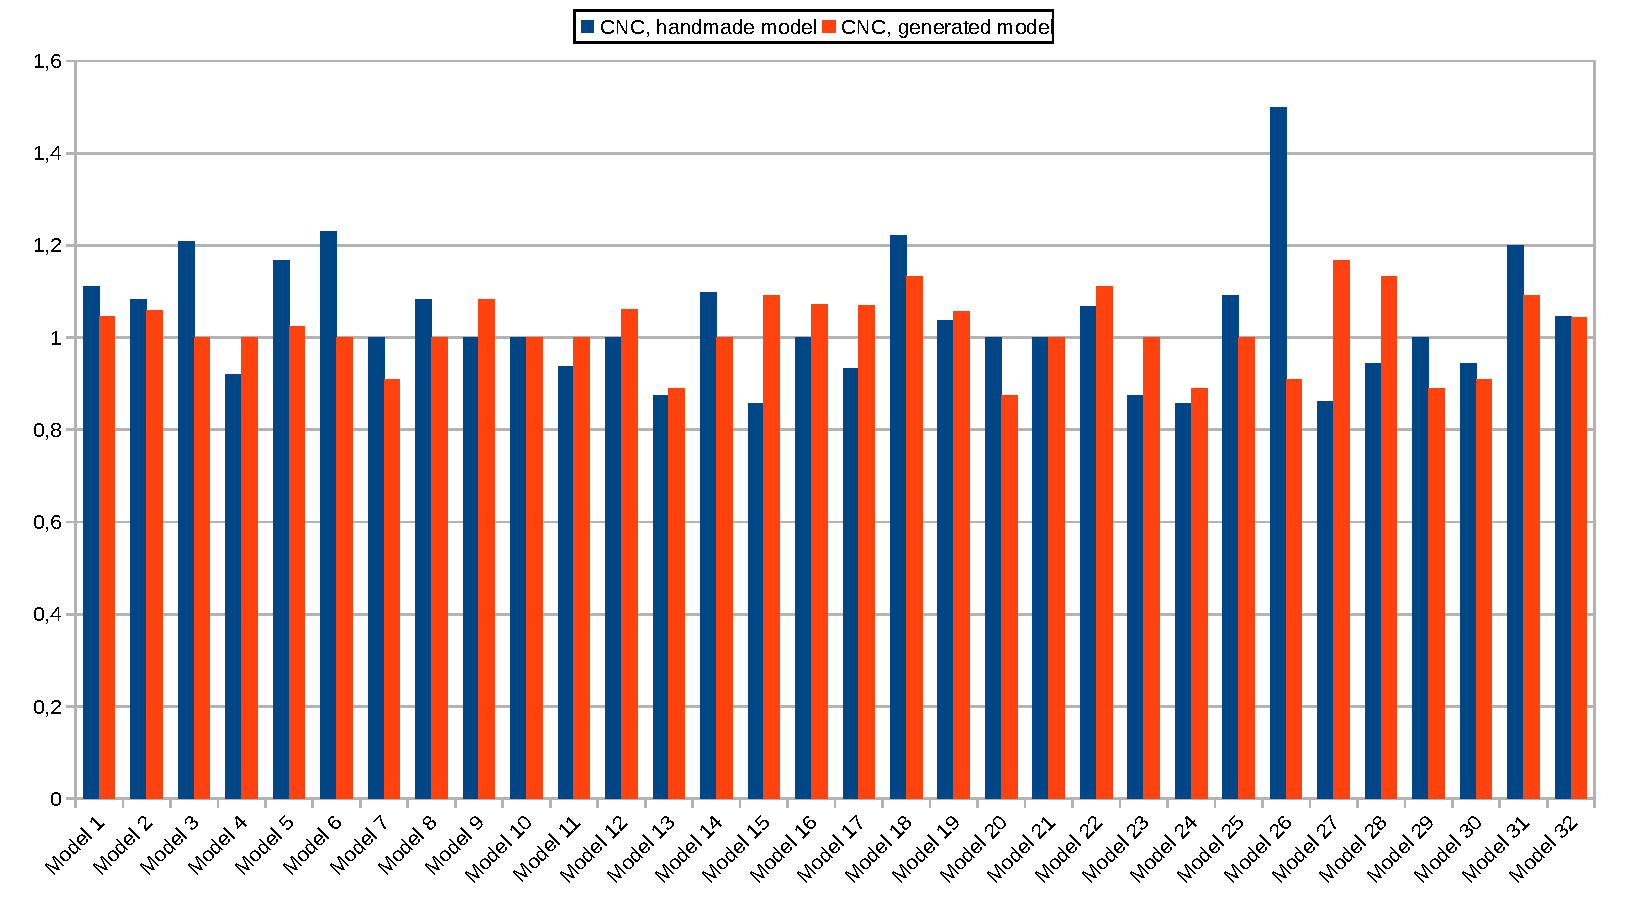
\includegraphics[width=0.95\textheight, angle=90]{./images/cnc_chart.pdf}
	\caption{Chart showing comparison of CNC metric between models}
	\label{bpmn:cnc_chart}
\end{figure}
\begin{figure}[p]
	\centering
	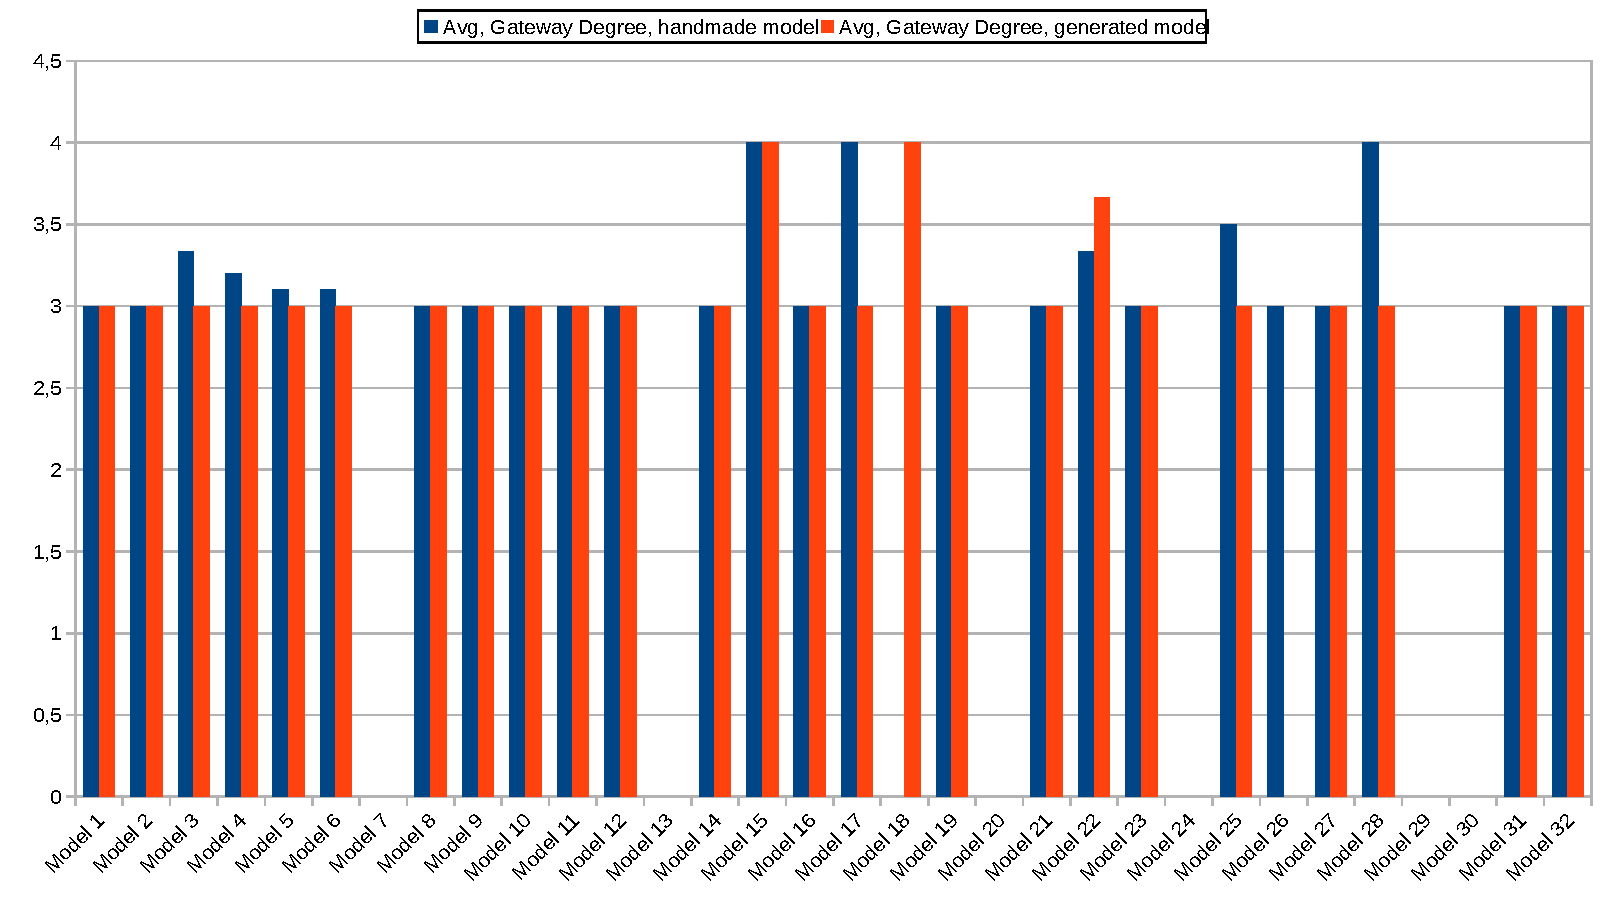
\includegraphics[width=0.95\textheight, angle=90]{./images/avg_chart.pdf}
	\caption{Chart showing comparison of Average Gateway Degree metric between models}
	\label{bpmn:avg_chart}
\end{figure}
\begin{figure}[p]
	\centering
	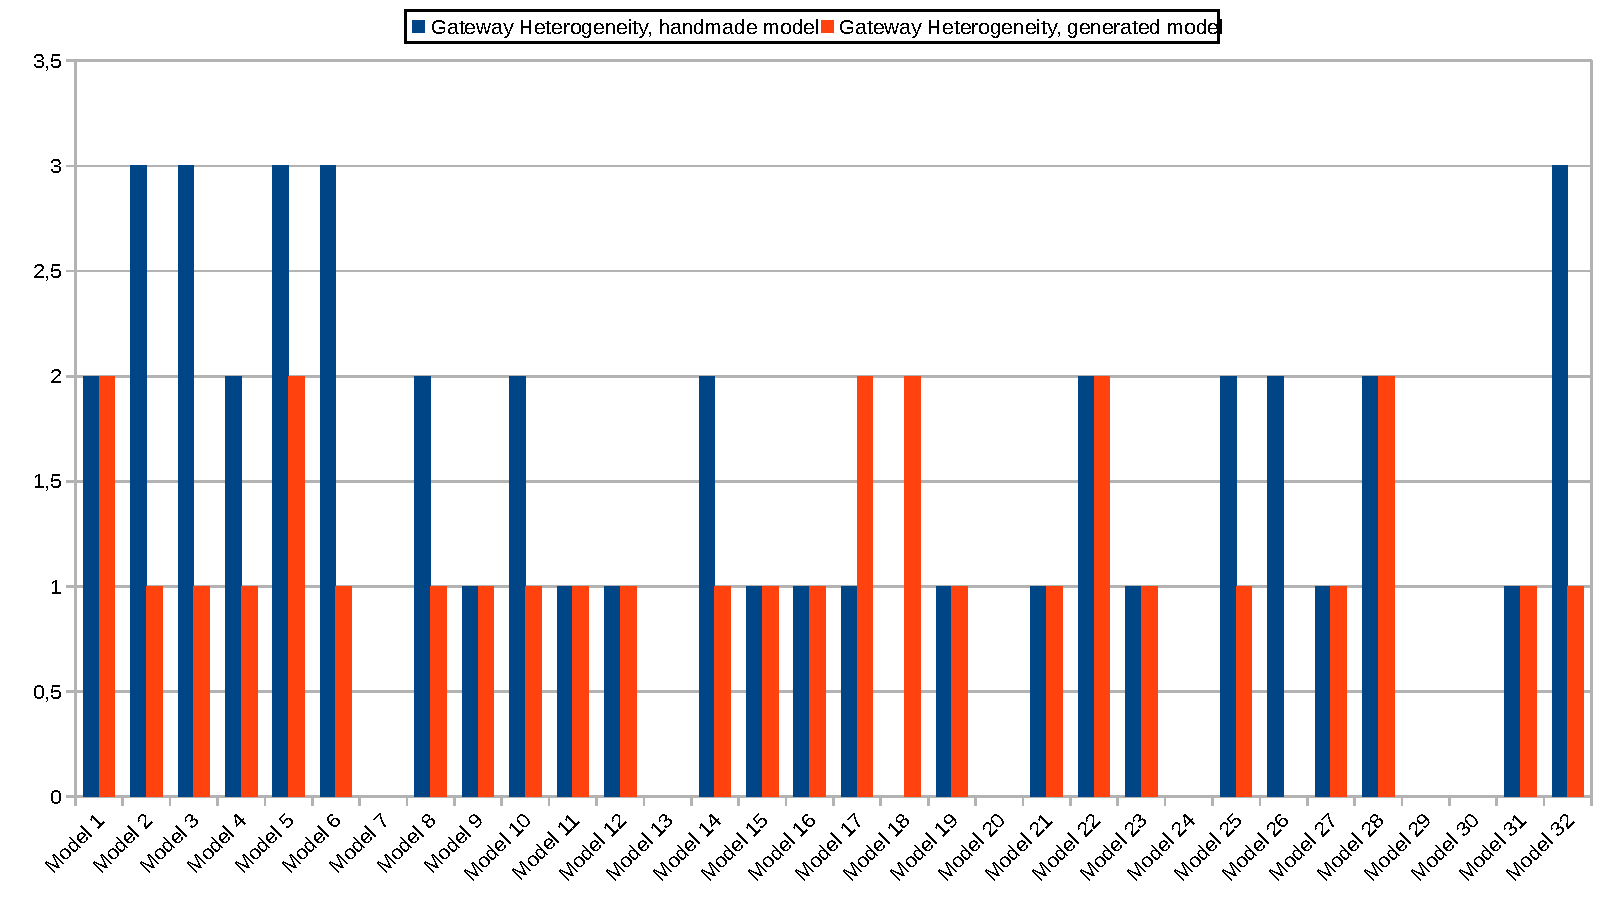
\includegraphics[width=0.95\textheight, angle=90]{./images/heter_chart.pdf}
	\caption{Chart showing comparison of Gateway Heterogeneity metric between models}
	\label{bpmn:heter_chart}
\end{figure}

\subsection{Detailed example analysis}
\label{sec:detailed-example}
In this section, a detailed analysis of a few models will be performed. This analysis will focus on generated results and the overall usability of automatically created models -- whether those capture the proper process flow from generated text and provide the useful BPMN diagrams.\\
Models number three, five and eighteen were chosen for detailed analysis. This choice of test models subset was based on the complexity metrics analysis described in previous section. Models number five and eighteen appeared a few times as a models extreme values of analysed metrics. Model number three was chosen due to the fact that its metrics values do not differentiate much from hand-made model, so it might be worthy to perform the detailed comparison and to analyse the differences that are not visible after metrics evaluation.

\subsubsection{Model 3}
\begin{tcolorbox}[
	breakable,
	arc=0mm,
	left=1pt,
	right = 1pt,
	boxrule=0mm,
	colback = {white},
	]
	\texttt{\input{./models/model3.txt}}
\end{tcolorbox}
\captionof{textdesc}{Text description for model number three}\label{txt:model3_val}
Text describes a process of taking order from guest at exclusive hotel. The described process can be separated into two parts -- registering the order by room-service manager and fulfilling it by waiter.\\
Table~\ref{csv:model3_val} shows the spreadsheet-based description of the extracted model, Figures~\ref{bpmn:generated_model3_val} and~\ref{bpmn:model3_val} present the generated BPMN diagram and corresponding hand-made model.

{\scriptsize
	\begin{longtable}{|p{0.03 \hsize}|p{0.25 \hsize}|p{0.15 \hsize}|p{0.2 \hsize}|p{0.1 \hsize}|p{0.1 \hsize}|}
		\hline
		Order & Activity & Condition & Who & Subprocess & Terminated.
		\\\hline\hline
		\csvreader[late after line=\\\hline]
		{./results/model3_intermediate_model.csv}
		{Order=\Order,Activity=\Activity,Condition=\Condition,Who=\Who,Subprocess=\Subprocess,Terminated=\Terminated}
		{\Order & \Activity & \Condition & \Who & \Subprocess & \Terminated}
		\caption{Spreadsheet-based description for process model number three}
		\label{csv:model3_val}
	\end{longtable}
}

\begin{figure}[H]
	\centering
	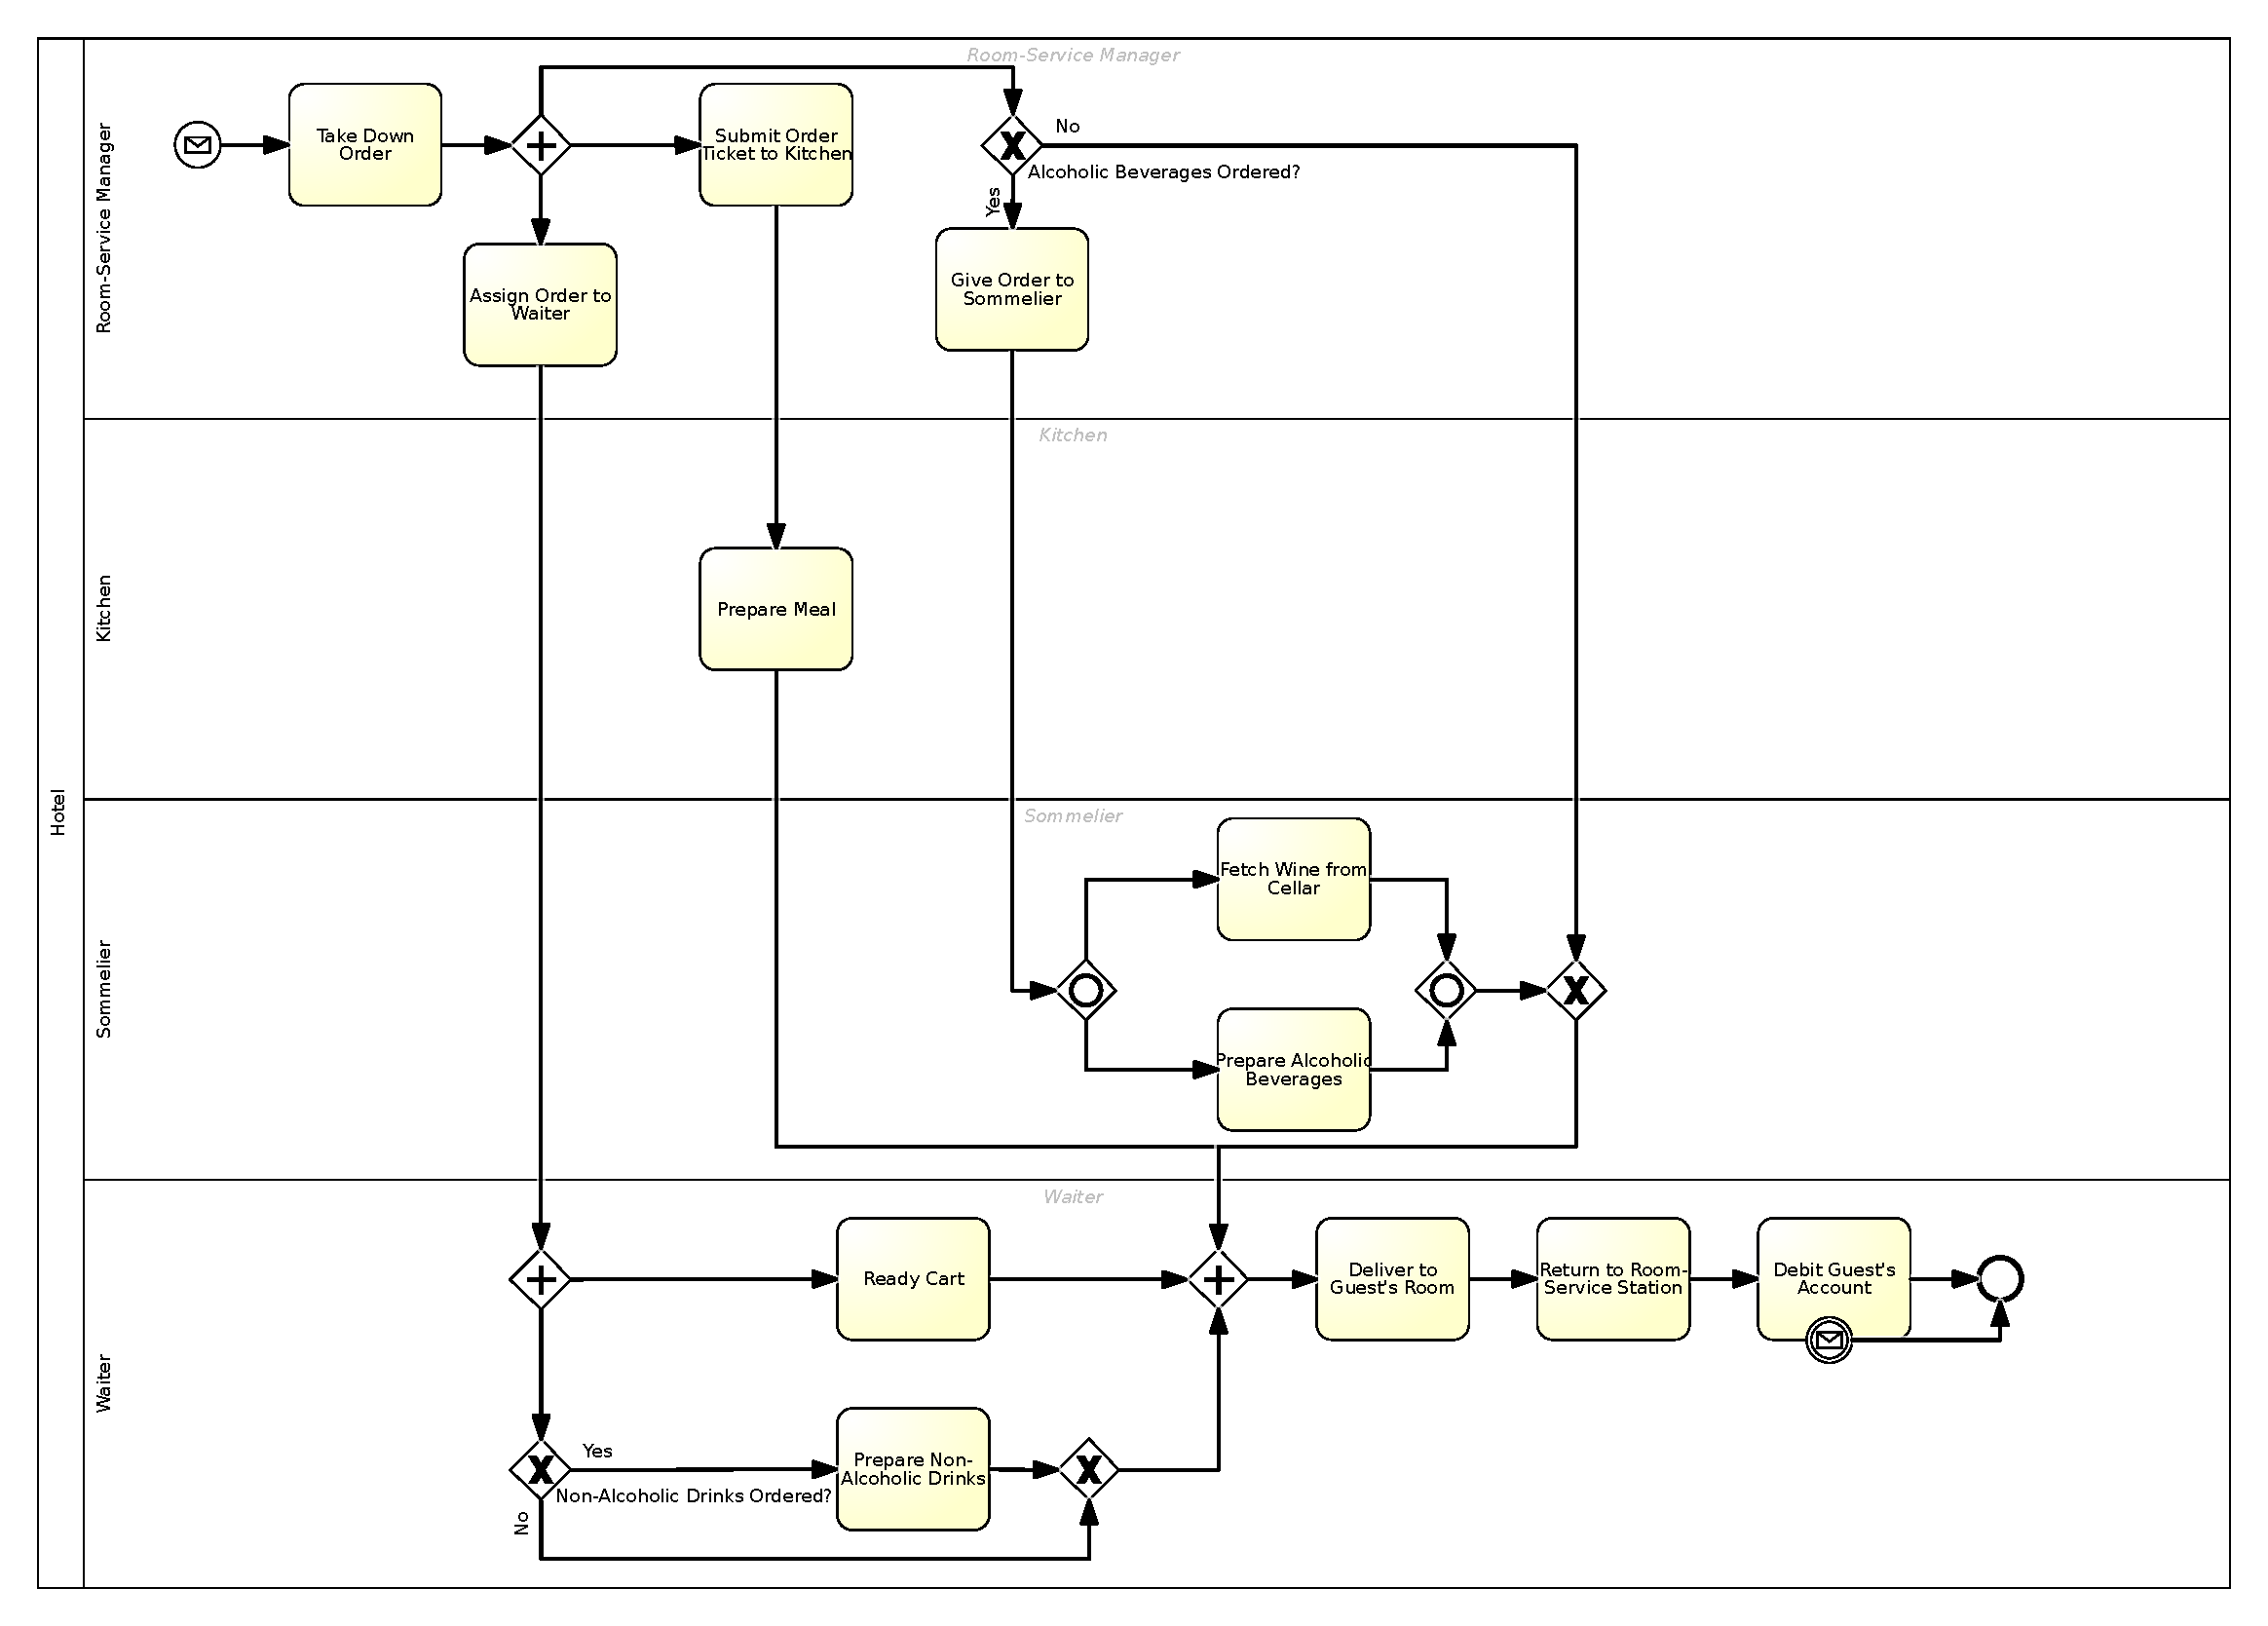
\includegraphics[width=0.95\textheight, angle=90]{./bpmn/model3.pdf}
	\caption{Hand-made BPMN diagram for process model number three}
	\label{bpmn:model3_val}
\end{figure}

\begin{figure}[H]
	\centering
	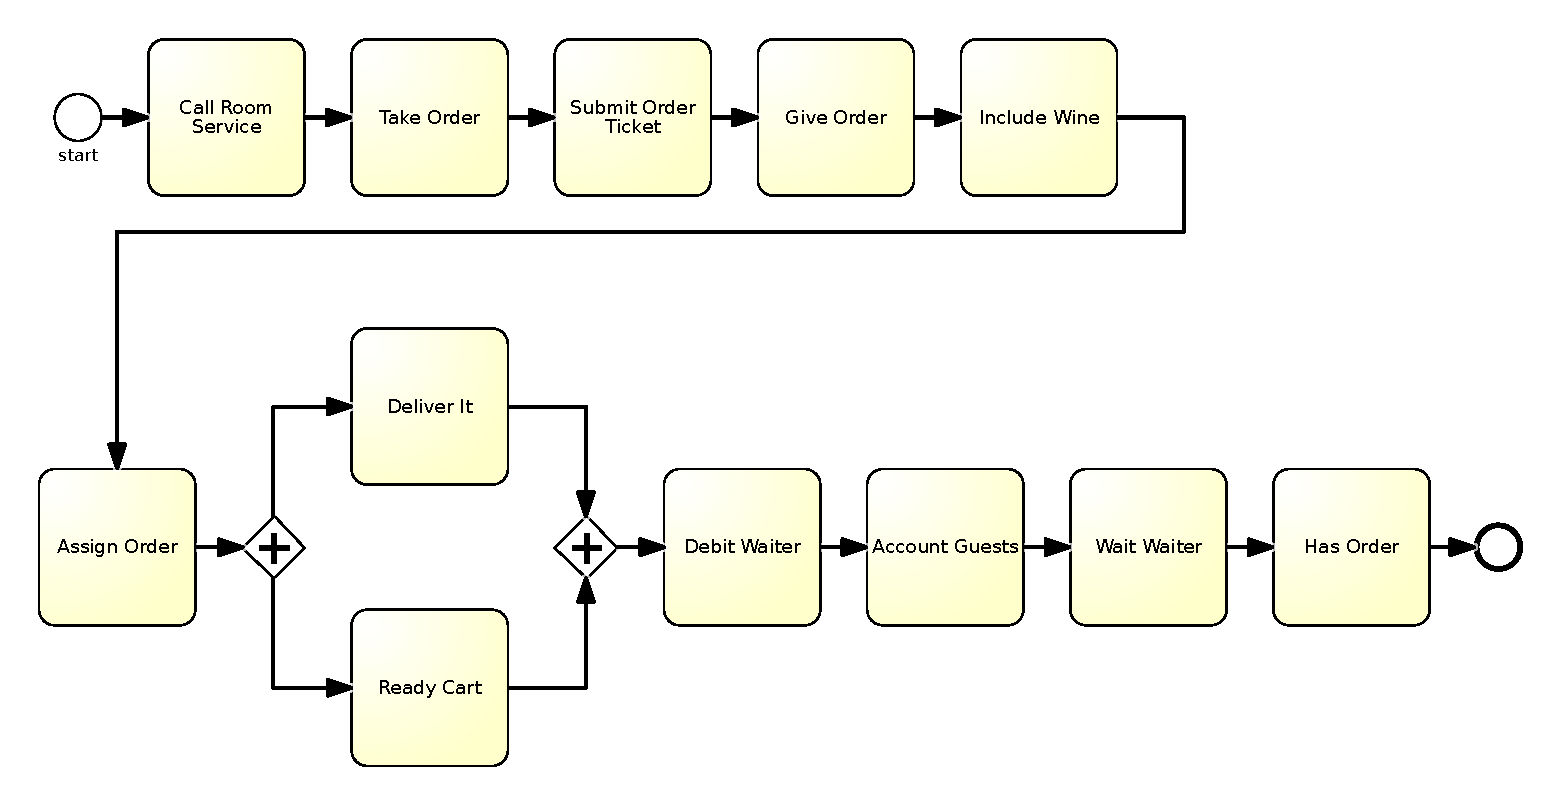
\includegraphics[width=\hsize]{./generated_bpmn/model3.pdf}
	\caption{BPMN diagram for process model number three generated from spreadsheet-based model}
	\label{bpmn:generated_model3_val}
\end{figure}

Unfortunately, the generated model is missing the pool and lanes elements, but this came from the fact, that current version of \emph{bpmn\_python} does not support the manual creation of those elements. On the other hand, the intermediate model shows that for some activities the \emph{``Who''} column was filled with correct information. In case of room-service manager the information about Participant that performs the activities is missing, due to the fact that room-service manager was addressed by a pronoun \emph{``She''}. The implemented method is unable to correctly identify actors described by pronouns and thus fails to provide correct information.\\
The first part of described process was extracted quite well -- the activities performed by room-service manager are correctly ordered. Few of the activities are missing information about the recipients of task result -- for example the activity \emph{``Submit Order Ticket''} omits the information that ticket is submitted to the kitchen.\\
The part of the process performed by waiter was more problematic. The algorithm created an incorrect parallel gateway which informs that waiter simultaneously prepares and delivers the cart, which is obviously incorrect. Several parts of description was not processed into activities -- while the part about kitchen and sommelier \emph{``doing their tasks''}, the information about waiter returning to the station was not extracted. This might be caused by the fact that verb \emph{``return''} was given in the gerund form as \emph{``returning''}. The phrase \emph{``the waiter debits the guest account''} was divided into two activities, because SpaCy parser failed to identify word \emph{``account''} as a noun and not a verb.\\
Comparing the results with hand-made model, it is apparent that latter correctly adds the activities performed by kitchen and sommelier. Also the control flow elements capture the described flow of actions in consecutive phases.

\subsubsection{Model 5}
\begin{tcolorbox}[
	breakable,
	arc=0mm,
	left=1pt,
	right = 1pt,
	boxrule=0mm,
	colback = {white},
	]
	\texttt{\input{./models/model5.txt}}
\end{tcolorbox}
\captionof{textdesc}{Text description for model number five}\label{txt:model5_val}
This process description is one of the largest from data set. The implemented method produced a process model with large number of activities involved. On the other hand, the hand-made counterpart has significantly lower number of activities, but includes higher number of control flow elements. Table~\ref{csv:model5_val} shows the spreadsheet-based description of extracted model, Figures~\ref{bpmn:generated_model5_val} and~\ref{bpmn:model5_val} presents the generated BPMN diagram and corresponding hand-made model.

{\scriptsize
	\begin{longtable}{|p{0.03 \hsize}|p{0.25 \hsize}|p{0.15 \hsize}|p{0.2 \hsize}|p{0.1 \hsize}|p{0.1 \hsize}|}
		\hline
		Order & Activity & Condition & Who & Subprocess & Terminated.
		\\\hline\hline
		\csvreader[late after line=\\\hline]
		{./results/model5_intermediate_model.csv}
		{Order=\Order,Activity=\Activity,Condition=\Condition,Who=\Who,Subprocess=\Subprocess,Terminated=\Terminated}
		{\Order & \Activity & \Condition & \Who & \Subprocess & \Terminated}
		\caption{Spreadsheet-based description for process model number five}
		\label{csv:model5_val}
	\end{longtable}
}
Comparison of the generated model with hand-made one shows that the implemented method lacks the ability to recognize some of the actions described in text as an event rather than activities. Tasks like \emph{``Create Notification''}, \emph{``Create Request''} and \emph{``Send message''} could be represented as message events. Also, the analysis of process model generated from model number five description shows that gateway extraction method fails to recognize more complex cases, which can appear in natural language. Consider the excerpt from process description, shown as Text~\ref{txt:model5_excerpt}:
\begin{tcolorbox}[
	breakable,
	arc=0mm,
	left=1pt,
	right = 1pt,
	boxrule=0mm,
	colback = {white},
	]
	\texttt{
		An electronic service then determines the significance of the customer based on information that has
		been collected during the history of the contractual relationship. In case the customer is premium, the
		process will link to an extra problem fix process (this process will not be detailed here). In case the
		customer is of certain significance which would affect the counter measures previously decided upon,
		the process goes back to re-prioritize these measures otherwise the process continues.	
	}
\end{tcolorbox}
\captionof{textdesc}{Excerpt of process description for model number five}\label{txt:model5_excerpt}
For a human modeller it is obvious that this text describes some form of conditional process flow, but it is not easy to process for machine. It might be possible to use longer phrases, like \emph{``In case of''} or \emph{``For the case that''} to signalize the possible presence of conditional flow, but there are probably a number of such phrases and identifying all of them might be a difficult task. The implemented method also had a problem with correct extraction of gateway conditions. In case of inclusive gateway added to the model, the gateway has two conditions \emph{``Problems are detected''} and \emph{``Problem is detected''}. This confusing description came from the fact, that word \emph{``no''} was labelled determiner (dependency tag ``det'') and not as a negation modifier -- thus it was omitted from condition name.

\begin{figure}[h!p]
	\centering
	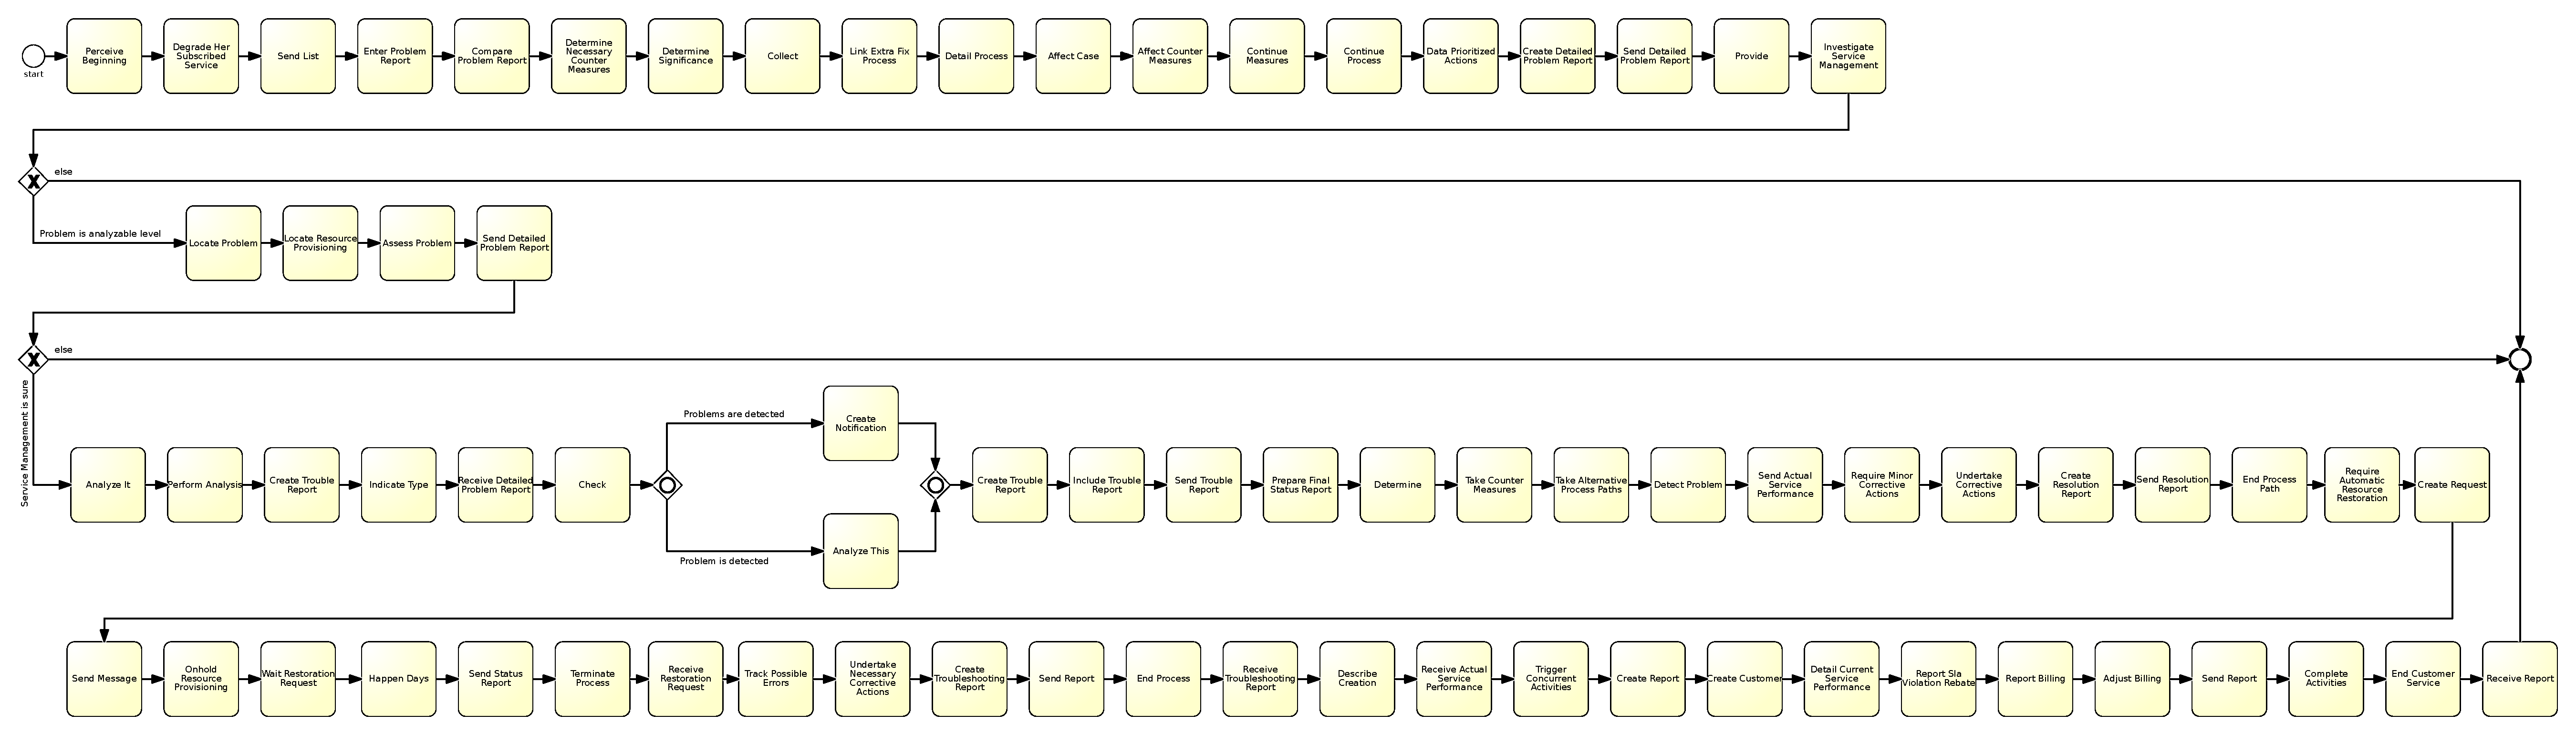
\includegraphics[width=0.90\textheight, angle=90]{./generated_bpmn/model5.pdf}
	\caption{BPMN diagram for process model number five generated from spreadsheet-based model (picture available at \url{https://github.com/KrzyHonk/nl-description-to-bpmn/tree/master/generated_bpmn})}
	\label{bpmn:generated_model5_val}
\end{figure}

\begin{figure}[h!p]
	\centering
	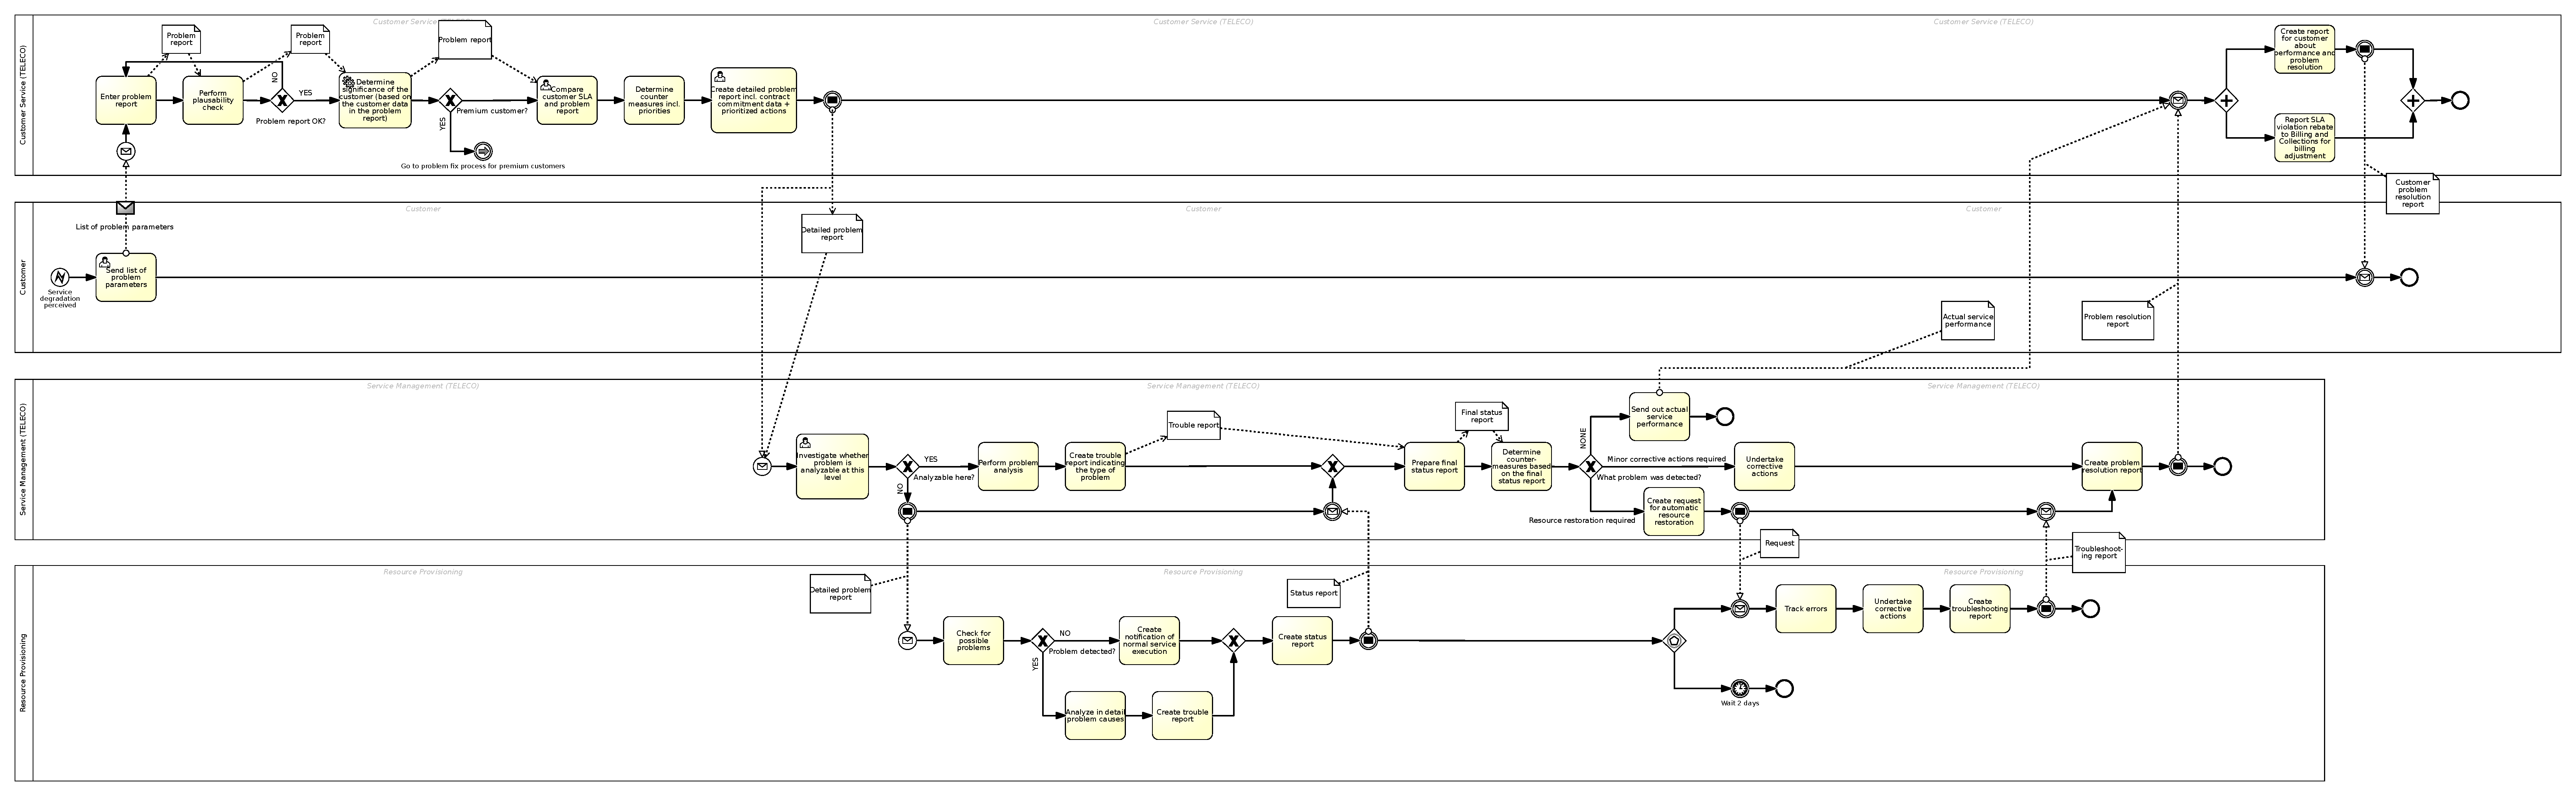
\includegraphics[width=0.90\textheight, angle=90]{./bpmn/model5.pdf}
	\caption{Hand-made BPMN diagram for process model number five (picture available at \url{https://github.com/KrzyHonk/nl-description-to-bpmn/tree/master/manual_bpmn})}
	\label{bpmn:model5_val}
\end{figure}

\subsubsection{Model 18}
\begin{tcolorbox}[
	breakable,
	arc=0mm,
	left=1pt,
	right = 1pt,
	boxrule=0mm,
	colback = {white},
	]
	\texttt{\input{./models/model18.txt}}
\end{tcolorbox}
\captionof{textdesc}{Text description for model number eighteen}\label{txt:model18_val}

{\scriptsize
	\begin{longtable}{|p{0.03 \hsize}|p{0.25 \hsize}|p{0.15 \hsize}|p{0.2 \hsize}|p{0.1 \hsize}|p{0.1 \hsize}|}
		\hline
		Order & Activity & Condition & Who & Subprocess & Terminated.
		\\\hline\hline
		\csvreader[late after line=\\\hline]
		{./results/model18_intermediate_model.csv}
		{Order=\Order,Activity=\Activity,Condition=\Condition,Who=\Who,Subprocess=\Subprocess,Terminated=\Terminated}
		{\Order & \Activity & \Condition & \Who & \Subprocess & \Terminated}
		\caption{Spreadsheet-based description for process model number eighteen}
		\label{csv:model18_val}
	\end{longtable}
}

\begin{figure}[h!p]
\centering
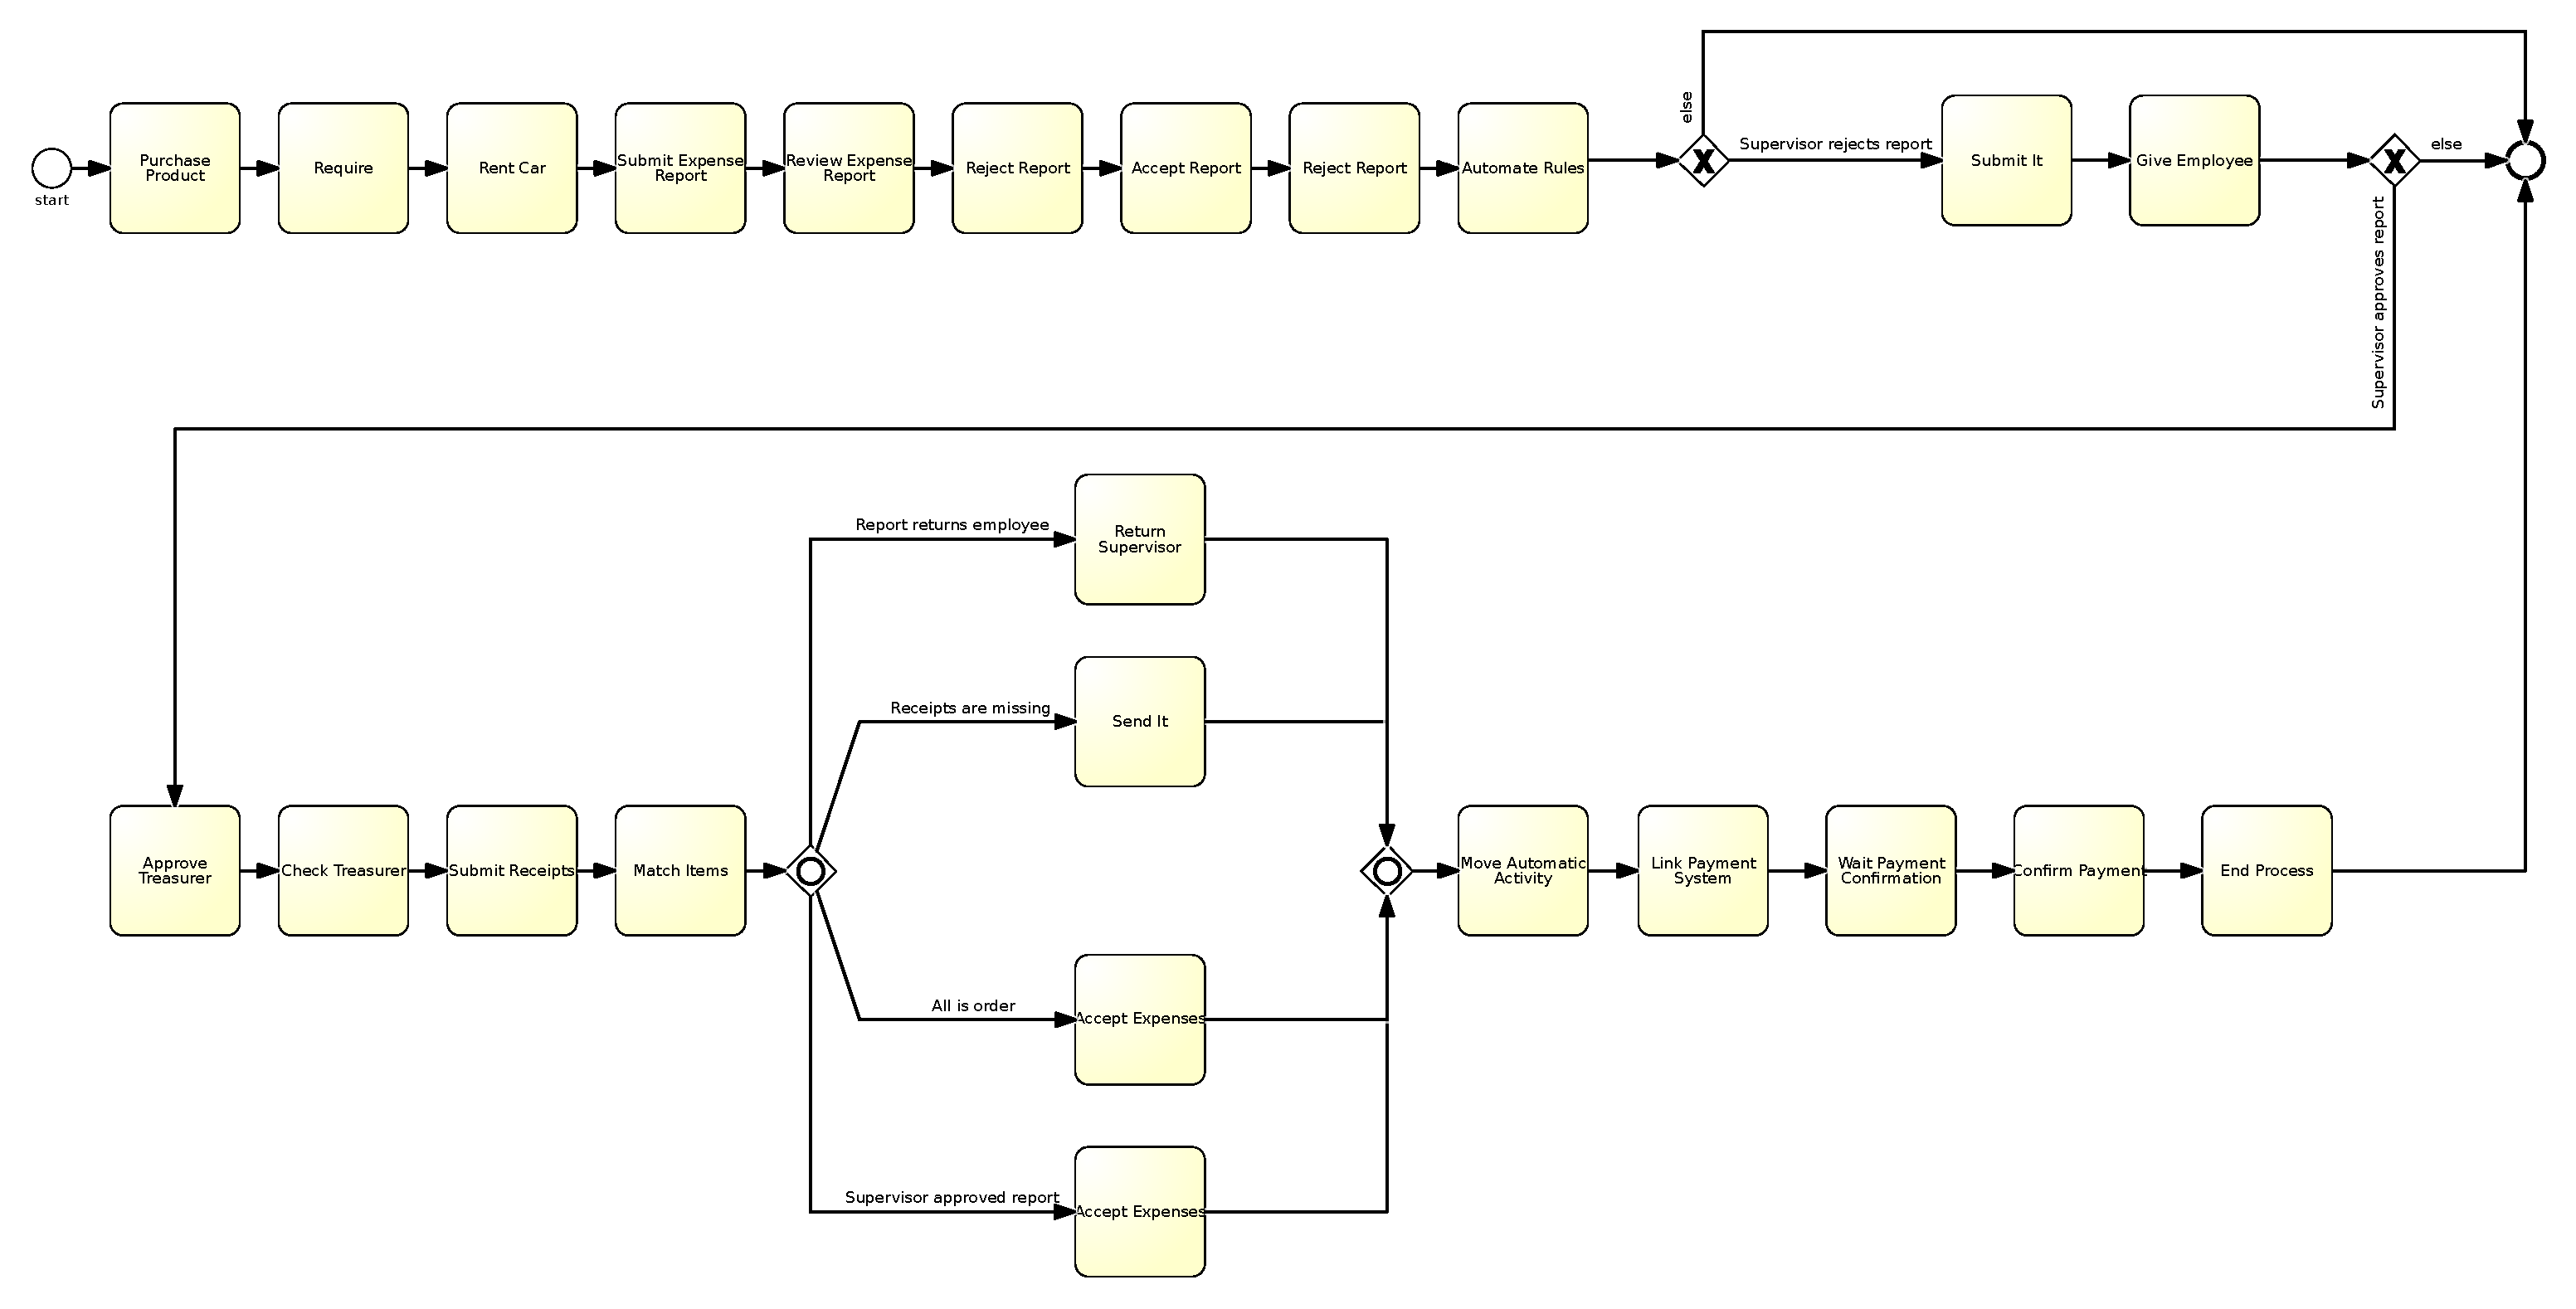
\includegraphics[width=\hsize]{./generated_bpmn/model18.pdf}
\caption{BPMN diagram for process model number eighteen generated from spreadsheet-based model}
\label{bpmn:generated_model18_val}
\end{figure}

\begin{figure}[h!p]
	\centering
	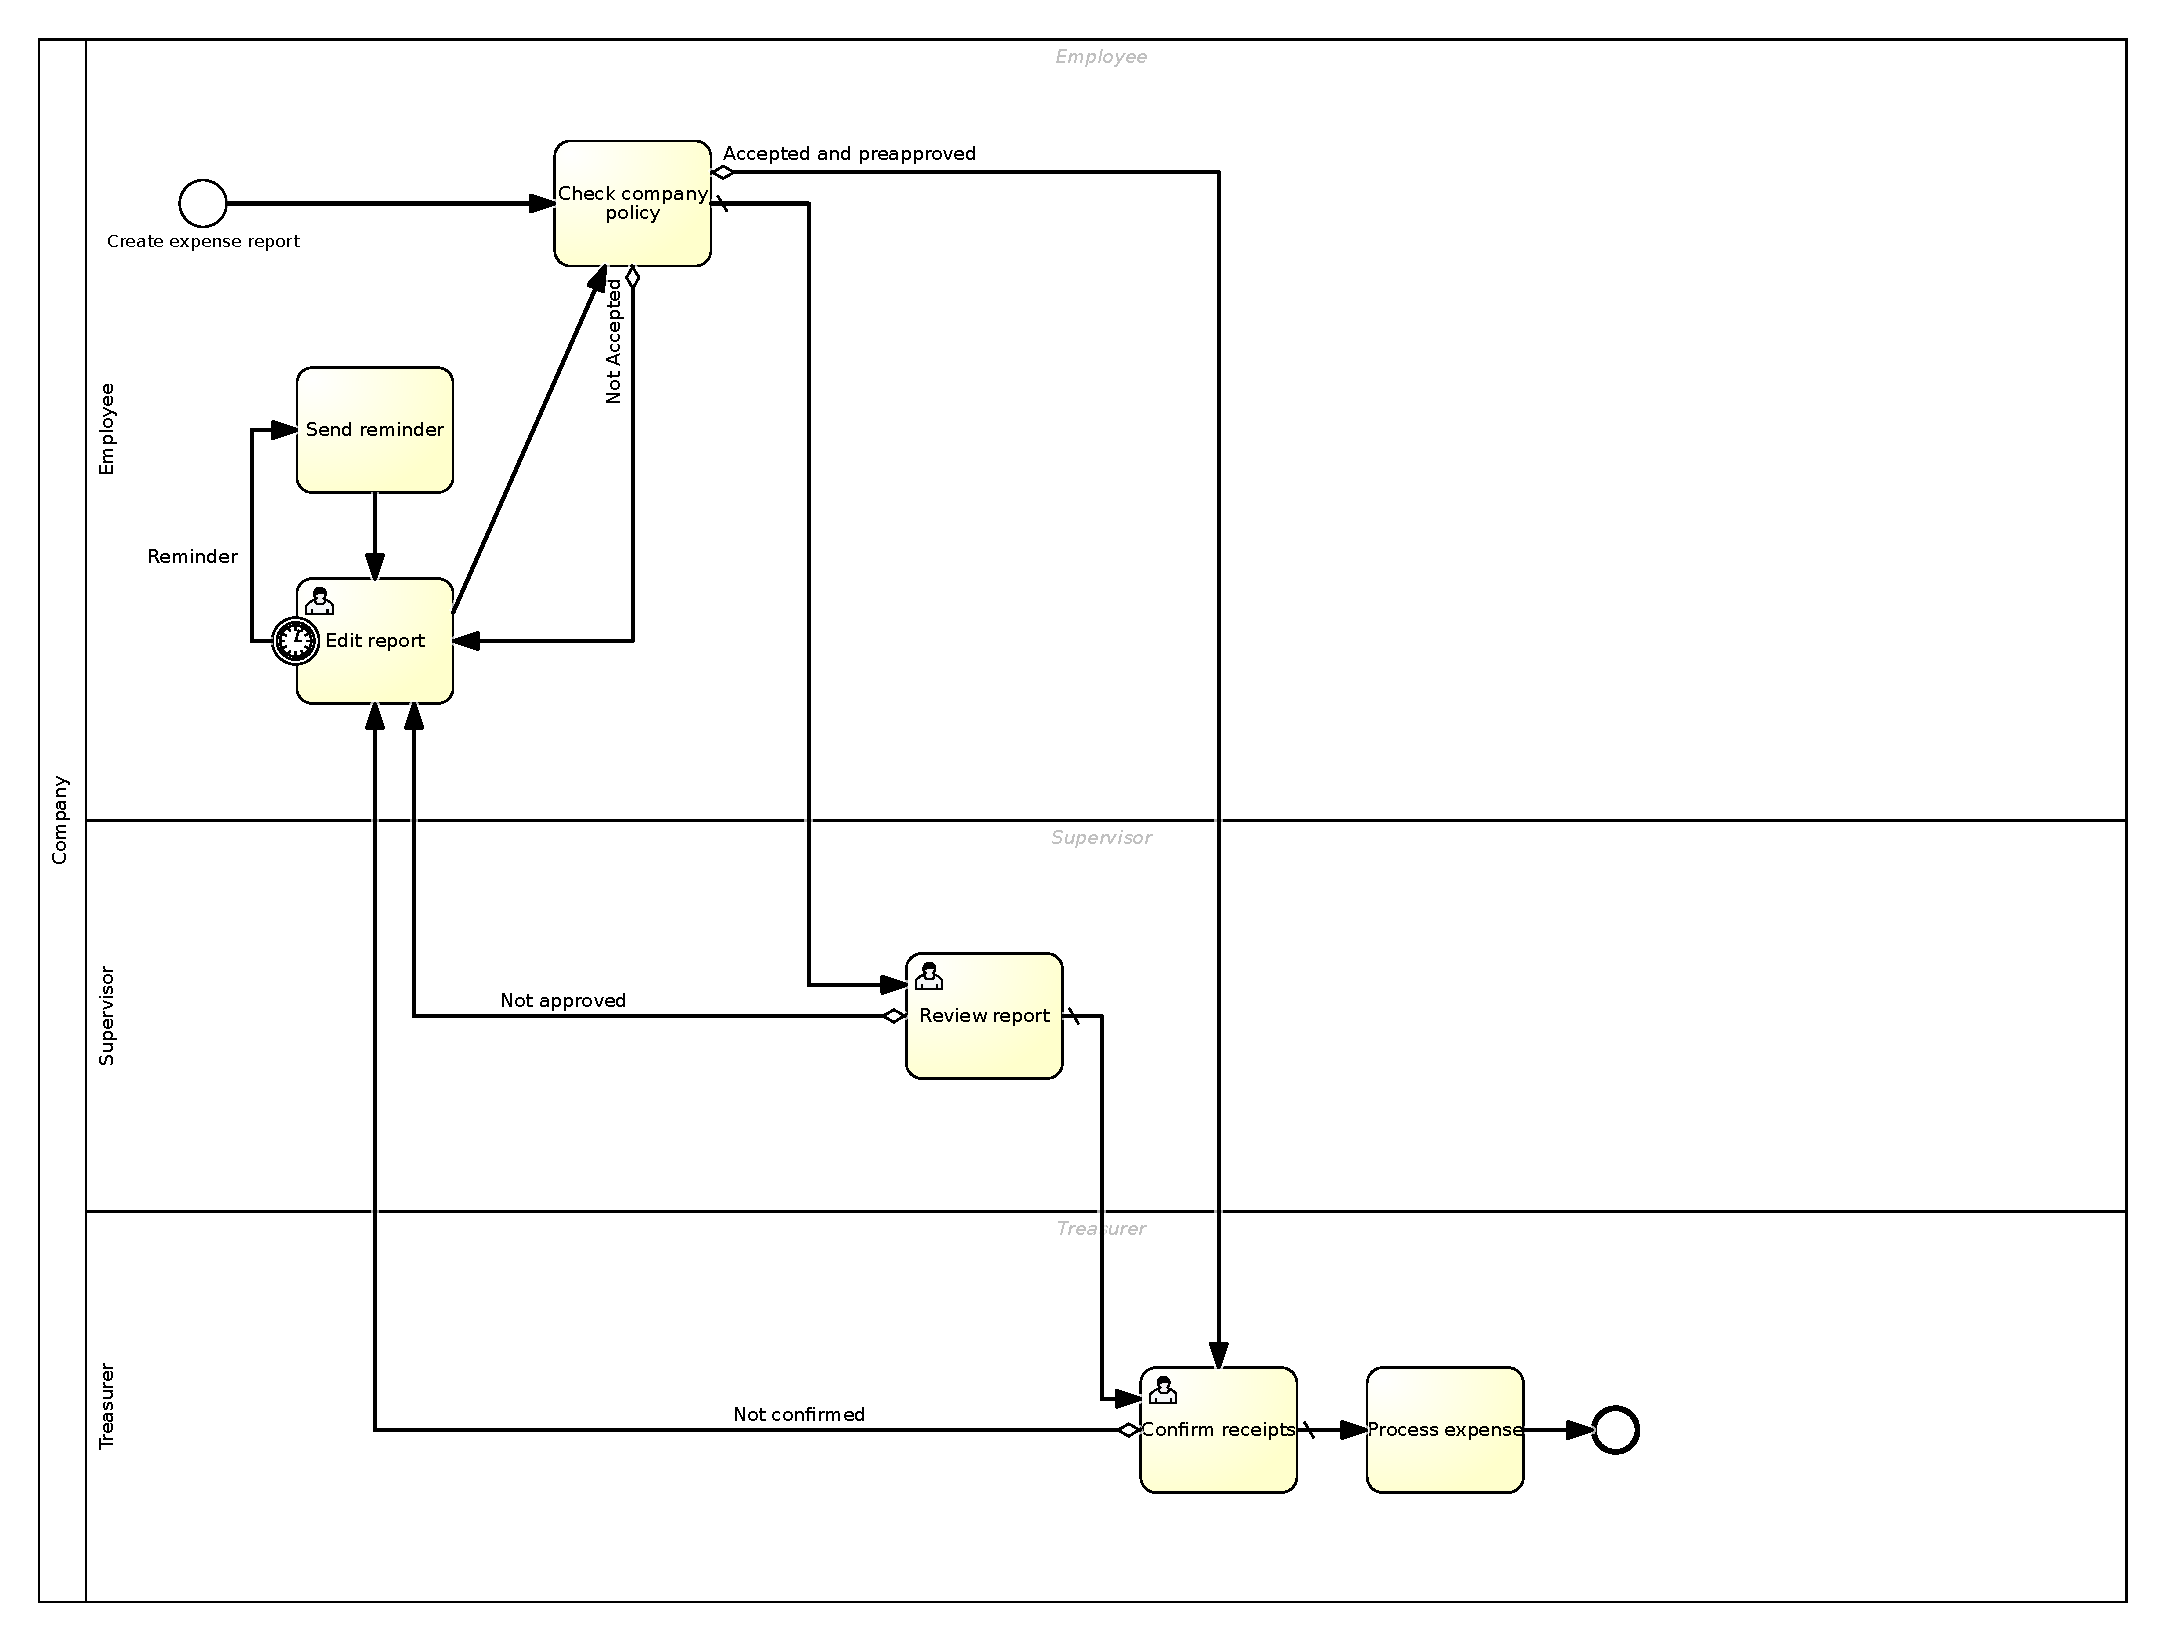
\includegraphics[width=\hsize]{./bpmn/model18.pdf}
	\caption{Hand-made BPMN diagram for process model number eighteen}
	\label{bpmn:model18_val}
\end{figure}

Like in the previous case, the model generated from this description has higher number of the activities, compared to the hand-made model. In this case, the reason is the fact that process description includes parts that do not describe an activities involved in the process, but rather add some additional information about process itself. Consider those parts shown as Texts~\ref{txt:model18_excerpt_one} and~\ref{txt:model18_excerpt_two}:
\begin{tcolorbox}[
	breakable,
	arc=0mm,
	left=1pt,
	right = 1pt,
	boxrule=0mm,
	colback = {white},
	]
	\texttt{
		An employee purchases a product or service he requires. For instance, a sales person on
		a trip rents a car.	
	}
\end{tcolorbox}
\captionof{textdesc}{First excerpt of process description for model number eighteen}\label{txt:model18_excerpt_one}
\begin{tcolorbox}[
	breakable,
	arc=0mm,
	left=1pt,
	right = 1pt,
	boxrule=0mm,
	colback = {white},
	]
	\texttt{
		Since the company has expense rules, there are circumstances where
		the supervisor can accept or reject the report upon first inspection. These rules could be
		automated, to reduce the workload on the supervisor.	
	}
\end{tcolorbox}
\captionof{textdesc}{Second excerpt of process description for model number eighteen}\label{txt:model18_excerpt_two}
The first excerpt provides an introduction for the described process case, the second excerpt gives an insight to the way in which the described company works. Both excerpts do not describe the actual process flow and while it is easy to recognize this for a human, a machine translation algorithm does not have the knowledge required to identify such cases. The presented method simply processes such information and create unnecessary activities (\emph{``Rent Car''}, \emph{``Automate Rules'}) from those excerpts. Overcoming this obstacle might be a challenging task.

\section{Method limitations}
The evaluation of implemented method of generating business process model from natural language description pointed out a number of limitations of implemented prototype. The most important of those limitations are:
\begin{itemize}
	\item adding only tasks and gateways to resulting model -- in some cases adding an intermediate event instead of the task might provide a better representation of a described process. The simplest way to solve this problem might be to add additional layer of SVO validation, which would check the verb included in SVO against a set of designated keywords. Examples of such keywords might be \emph{``send''} or \emph{``report''} (if identified as a verb) -- if SVO consists such a verb, it might be better to represent it as an intermediate message event, rather than a task,
	\item the proposed method for gateway extraction is unable to recognize more complex cases of conditional flow -- those can be signalized by specific phrases, such as \emph{``In case of''}, \emph{``For the case that''} and others,
	\item if the description consists some information that are not a part of process flow, it will be also incorporated into the created BPMN. While this problem might be impossible to overcome by improving the algorithm (machine do not understand the context of processed text), it might be a good idea to incorporate a lightweight standardization to the text and require that description covers only information about process flow,
	\item identifying the actual actors in the process, that were addressed by pronoun word (\emph{``I''}, \emph{``He''}, \emph{``She''}). This is a problem known as a anaphora resolution, and it is already covered in multiple sources~(\cite{anaphora-hale},~\cite{anaphora-kotek}). Implementing a solution for anaphora resolution might improve results of process generation -- with this, it might be possible to identify an actor for every activity in a process and enhance the generated model with pools and lanes.
\end{itemize}
This section described the validation methodology applied to implemented prototype and presented the validation results. Also, the proposed methodology limitations were highlighted. Next section summarises the proposed approach and concludes this work.